\documentclass{standalone}

\usepackage{tikz}
\usetikzlibrary{arrows,backgrounds,er,chains}

\begin{document}
  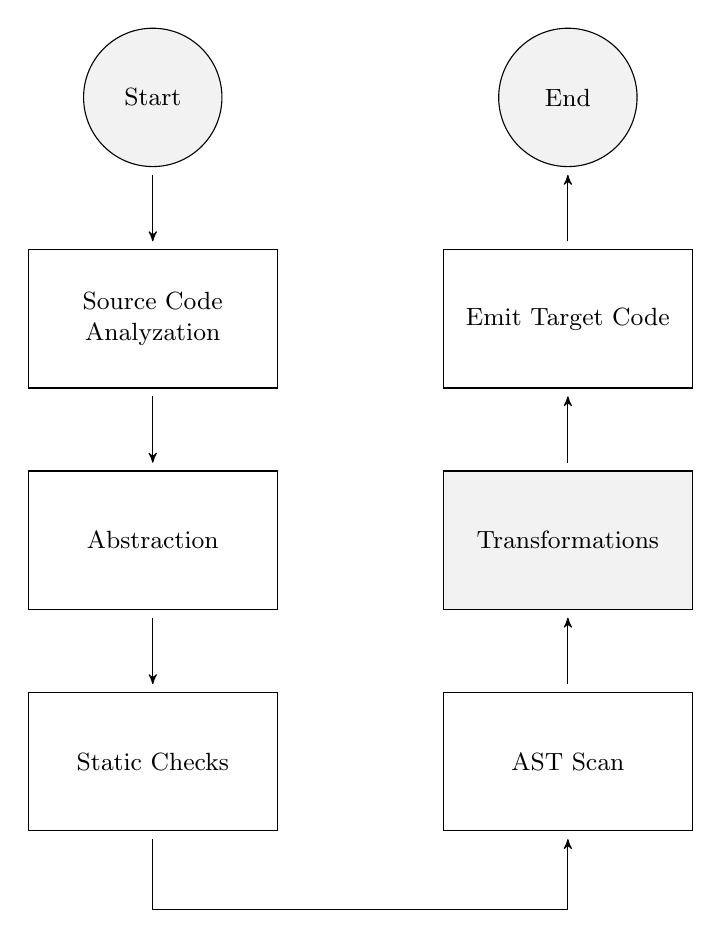
\begin{tikzpicture}[
    ->,
    >=stealth',
    shorten >= 1pt,
    auto,
    node distance=3em and 6em,
    font=\small,
    text centered,
    every entity/.style={
      minimum width=9em,
  	  minimum height=5em,
      outer sep=0,
      inner ysep=.5em
    }
    ]
    
    \node [entity] (A) [draw=none, fill=none] {};
    \node at (A.center) [circle] (a) [draw, fill=gray!10, inner sep=1em, minimum size=5em] {Start};

    \node [entity] (B) [below = of A] {\begin{tabular}{c}Source Code \\ Analyzation\end{tabular}};
    \node [entity] (C) [below = of B] {Abstraction};
    \node [entity] (D) [below = of C] {Static Checks};
    \node [entity] (E) [right = of D] {AST Scan};
    \node [entity] (F) [above = of E, fill=gray!10] {Transformations};
    \node [entity] (G) [above = of F] {Emit Target Code};
    
    \node [entity] (H) [above = of G, draw=none, fill=none] {};
    \node at (H.center) [circle] (h) [draw, fill=gray!10, inner sep=1em, minimum size=5em] {End};

    \path[shorten >=0.3em,shorten <=0.3em,->] (A) edge node {} (B);
    \path[shorten >=0.3em,shorten <=0.3em,->] (B) edge node {} (C);
    \path[shorten >=0.3em,shorten <=0.3em,->] (C) edge node {} (D);
    
    \draw[shorten >=0.3em,shorten <=0.3em,->] (D.south) -- ++(0,-1) -|  (E.south);
    
    \path[shorten >=0.3em,shorten <=0.3em,->] (E) edge node {} (F);
    \path[shorten >=0.3em,shorten <=0.3em,->] (F) edge node {} (G);
    \path[shorten >=0.3em,shorten <=0.3em,->] (G) edge node {} (H);
    
  \end{tikzpicture}
\end{document}
